\documentclass{article}
\usepackage{tikz}

\begin{document}

\begin{tikzpicture}[scale=0.5]
    % Piano keys
    \foreach \x in {1,...,88} {
        \draw[fill=yellow!\x!white] (\x,-2) rectangle ++(1,3);
    }
    \foreach \x in {1,...,88} {
        \draw[fill=black] (\x,-2) rectangle ++(1,1);
    }

    % Note labels
    \foreach \x in {1,...,88} {
        \node at (\x,-1) {\textcolor{white}{\textbf{\textit{\ifodd\x\else\fi\note}}}};
    }

    % Background color
    \fill[yellow!20] (0,-2) rectangle (89,3);

    % Label border
    \draw[ultra thick, rounded corners=5pt] (0,-2) rectangle (89,3);

\end{tikzpicture}

\end{document}